% Seminar 3 - Page 9. Fragment for
% % Seminar 3 - Page 9. Fragment for
% % Seminar 3 - Page 9. Fragment for
% % Seminar 3 - Page 9. Fragment for
% \input{seminars/pages/seminar3-pagina9-en}; no preamble or page break.
% EDITORIAL NOTES:
% - The relation on plane lines is given in the manuscript as equality
%   or empty intersection (distinct parallel lines). Its form is retained.
% - The handwritten symbol for the upper semicircle appears to be B^1;
%   the superscript is slightly uncertain.
% - The manuscript defines B^1 by |z|=1 and Im(z)>=0, thereby including
%   both 1 and -1. The parametrisation t in [0,pi) excludes -1, so it
%   cannot be surjective onto B^1 as literally defined. Not silently fixed.
% - The stated intersection of the line through O with the semicircle
%   is likewise ambiguous for horizontal lines, when both endpoints
%   are included. An endpoint convention would resolve the discrepancy.
% - The geometric sketch and commuting triangle are redrawn with TikZ.
% - Exercises 1 and 2 have not been solved beyond the manuscript's text.
% - The boxed cardinal notation at the end is retained as written;
%   it is not a formal construction of a set of all equipotent sets.

\subsection*{Seminar 3 - Page 9}
\begingroup
\setlength{\abovedisplayskip}{5pt}
\setlength{\belowdisplayskip}{5pt}
\setlength{\abovedisplayshortskip}{3pt}
\setlength{\belowdisplayshortskip}{3pt}

Let $\mathcal D$ be the set of lines in the plane. Define
\[
 d_1\sim d_2\ \overset{\mathrm{def}}{\iff}\
 \begin{cases}
 d_1=d_2,\\[-2pt]
 \text{or}\\[-2pt]
 d_1\cap d_2=\varnothing.
 \end{cases}
\]
Show that $\sim$ is an equivalence relation on $\mathcal D$ and that
\[
 \mathcal D/{\sim}\ \cong\ [0,\pi).
\]

\noindent\underline{Proof.}
The manuscript considers an injective map
\[
 [0,\pi)\longrightarrow B^1,\qquad
 B^1=\{z\in\mathbb C\mid |z|=1,\ \operatorname{Im}(z)\geq 0\},
\]
\[
 t\longmapsto\cos t+i\sin t=e^{it}.
\]

\begin{center}
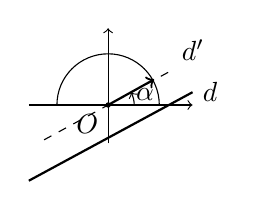
\begin{tikzpicture}[scale=0.65]
  \draw[->] (-1.55,0)--(1.65,0);
  \draw[->] (0,-0.75)--(0,1.50);
  \draw (-1,0) arc[start angle=180,end angle=0,radius=1];
  \draw[thick] (-1.55,-1.48)--(1.65,0.25) node[right] {$d$};
  \draw[dashed] (-1.25,-0.68)--(1.25,0.68) node[above right] {$d'$};
  \draw[->,thick] (0,0)--(0.9,0.5);
  \draw[->] (0.51,0) arc[start angle=0,end angle=29,radius=0.51];
  \node at (0.72,0.20) {$\alpha$};
  \fill (0,0) circle (1.5pt) node[below left] {$O$};
\end{tikzpicture}
\end{center}

\[
\begin{tikzcd}[column sep=large,row sep=large]
 \mathcal D\arrow[r,"p"]\arrow[d,"f"']
   & \mathcal D/{\sim}\arrow[dl,dashed,"\overline f"]\\
 B^1 &
\end{tikzcd}
\]
The map $f(d)$ is given as the intersection with $B^1$ of the line
through $O$ parallel to $d$.
The notes state
\[
 R_f=\sim,\qquad f\text{ is surjective},
\]
so there is a unique induced bijection
\[
 \exists!\,\overline f:\mathcal D/{\sim}\longrightarrow B^1,
 \qquad \overline f\text{ is bijective}.
\]

\medskip
\noindent\textbf{Exercise 1.}
Let $B\subseteq A$ be sets and define a relation on $\mathcal P(A)$ by
\[
 X\sim Y\iff X\cap B=Y\cap B.
\]
Show that $\sim$ is an equivalence relation and that
\[
 \mathcal P(A)/{\sim}\ \cong\ \mathcal P(B),
 \qquad X\longmapsto X\cap B.
\]

\noindent\textbf{Exercise 2.}
If $|M|=n$, calculate the number of equivalence relations
that can be defined on $M$.

\medskip
\noindent For sets $A,B$, define
\[
 A\sim B\ \overset{\mathrm{def}}{\iff}\
 \exists\,f:A\longrightarrow B\text{ bijective}.
\]
This is an equivalence relation (equipotence). The notes denote
cardinality by
\[
 \boxed{\widehat A\ \overset{\mathrm{not}}{=}
 \operatorname{card}(A)\ \overset{\mathrm{not}}{=}\ |A|}.
\]

\endgroup
; no preamble or page break.
% EDITORIAL NOTES:
% - The relation on plane lines is given in the manuscript as equality
%   or empty intersection (distinct parallel lines). Its form is retained.
% - The handwritten symbol for the upper semicircle appears to be B^1;
%   the superscript is slightly uncertain.
% - The manuscript defines B^1 by |z|=1 and Im(z)>=0, thereby including
%   both 1 and -1. The parametrisation t in [0,pi) excludes -1, so it
%   cannot be surjective onto B^1 as literally defined. Not silently fixed.
% - The stated intersection of the line through O with the semicircle
%   is likewise ambiguous for horizontal lines, when both endpoints
%   are included. An endpoint convention would resolve the discrepancy.
% - The geometric sketch and commuting triangle are redrawn with TikZ.
% - Exercises 1 and 2 have not been solved beyond the manuscript's text.
% - The boxed cardinal notation at the end is retained as written;
%   it is not a formal construction of a set of all equipotent sets.

\subsection*{Seminar 3 - Page 9}
\begingroup
\setlength{\abovedisplayskip}{5pt}
\setlength{\belowdisplayskip}{5pt}
\setlength{\abovedisplayshortskip}{3pt}
\setlength{\belowdisplayshortskip}{3pt}

Let $\mathcal D$ be the set of lines in the plane. Define
\[
 d_1\sim d_2\ \overset{\mathrm{def}}{\iff}\
 \begin{cases}
 d_1=d_2,\\[-2pt]
 \text{or}\\[-2pt]
 d_1\cap d_2=\varnothing.
 \end{cases}
\]
Show that $\sim$ is an equivalence relation on $\mathcal D$ and that
\[
 \mathcal D/{\sim}\ \cong\ [0,\pi).
\]

\noindent\underline{Proof.}
The manuscript considers an injective map
\[
 [0,\pi)\longrightarrow B^1,\qquad
 B^1=\{z\in\mathbb C\mid |z|=1,\ \operatorname{Im}(z)\geq 0\},
\]
\[
 t\longmapsto\cos t+i\sin t=e^{it}.
\]

\begin{center}
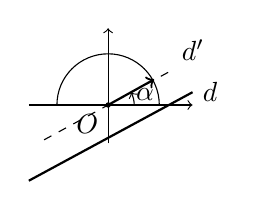
\begin{tikzpicture}[scale=0.65]
  \draw[->] (-1.55,0)--(1.65,0);
  \draw[->] (0,-0.75)--(0,1.50);
  \draw (-1,0) arc[start angle=180,end angle=0,radius=1];
  \draw[thick] (-1.55,-1.48)--(1.65,0.25) node[right] {$d$};
  \draw[dashed] (-1.25,-0.68)--(1.25,0.68) node[above right] {$d'$};
  \draw[->,thick] (0,0)--(0.9,0.5);
  \draw[->] (0.51,0) arc[start angle=0,end angle=29,radius=0.51];
  \node at (0.72,0.20) {$\alpha$};
  \fill (0,0) circle (1.5pt) node[below left] {$O$};
\end{tikzpicture}
\end{center}

\[
\begin{tikzcd}[column sep=large,row sep=large]
 \mathcal D\arrow[r,"p"]\arrow[d,"f"']
   & \mathcal D/{\sim}\arrow[dl,dashed,"\overline f"]\\
 B^1 &
\end{tikzcd}
\]
The map $f(d)$ is given as the intersection with $B^1$ of the line
through $O$ parallel to $d$.
The notes state
\[
 R_f=\sim,\qquad f\text{ is surjective},
\]
so there is a unique induced bijection
\[
 \exists!\,\overline f:\mathcal D/{\sim}\longrightarrow B^1,
 \qquad \overline f\text{ is bijective}.
\]

\medskip
\noindent\textbf{Exercise 1.}
Let $B\subseteq A$ be sets and define a relation on $\mathcal P(A)$ by
\[
 X\sim Y\iff X\cap B=Y\cap B.
\]
Show that $\sim$ is an equivalence relation and that
\[
 \mathcal P(A)/{\sim}\ \cong\ \mathcal P(B),
 \qquad X\longmapsto X\cap B.
\]

\noindent\textbf{Exercise 2.}
If $|M|=n$, calculate the number of equivalence relations
that can be defined on $M$.

\medskip
\noindent For sets $A,B$, define
\[
 A\sim B\ \overset{\mathrm{def}}{\iff}\
 \exists\,f:A\longrightarrow B\text{ bijective}.
\]
This is an equivalence relation (equipotence). The notes denote
cardinality by
\[
 \boxed{\widehat A\ \overset{\mathrm{not}}{=}
 \operatorname{card}(A)\ \overset{\mathrm{not}}{=}\ |A|}.
\]

\endgroup
; no preamble or page break.
% EDITORIAL NOTES:
% - The relation on plane lines is given in the manuscript as equality
%   or empty intersection (distinct parallel lines). Its form is retained.
% - The handwritten symbol for the upper semicircle appears to be B^1;
%   the superscript is slightly uncertain.
% - The manuscript defines B^1 by |z|=1 and Im(z)>=0, thereby including
%   both 1 and -1. The parametrisation t in [0,pi) excludes -1, so it
%   cannot be surjective onto B^1 as literally defined. Not silently fixed.
% - The stated intersection of the line through O with the semicircle
%   is likewise ambiguous for horizontal lines, when both endpoints
%   are included. An endpoint convention would resolve the discrepancy.
% - The geometric sketch and commuting triangle are redrawn with TikZ.
% - Exercises 1 and 2 have not been solved beyond the manuscript's text.
% - The boxed cardinal notation at the end is retained as written;
%   it is not a formal construction of a set of all equipotent sets.

\subsection*{Seminar 3 - Page 9}
\begingroup
\setlength{\abovedisplayskip}{5pt}
\setlength{\belowdisplayskip}{5pt}
\setlength{\abovedisplayshortskip}{3pt}
\setlength{\belowdisplayshortskip}{3pt}

Let $\mathcal D$ be the set of lines in the plane. Define
\[
 d_1\sim d_2\ \overset{\mathrm{def}}{\iff}\
 \begin{cases}
 d_1=d_2,\\[-2pt]
 \text{or}\\[-2pt]
 d_1\cap d_2=\varnothing.
 \end{cases}
\]
Show that $\sim$ is an equivalence relation on $\mathcal D$ and that
\[
 \mathcal D/{\sim}\ \cong\ [0,\pi).
\]

\noindent\underline{Proof.}
The manuscript considers an injective map
\[
 [0,\pi)\longrightarrow B^1,\qquad
 B^1=\{z\in\mathbb C\mid |z|=1,\ \operatorname{Im}(z)\geq 0\},
\]
\[
 t\longmapsto\cos t+i\sin t=e^{it}.
\]

\begin{center}
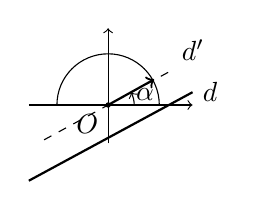
\begin{tikzpicture}[scale=0.65]
  \draw[->] (-1.55,0)--(1.65,0);
  \draw[->] (0,-0.75)--(0,1.50);
  \draw (-1,0) arc[start angle=180,end angle=0,radius=1];
  \draw[thick] (-1.55,-1.48)--(1.65,0.25) node[right] {$d$};
  \draw[dashed] (-1.25,-0.68)--(1.25,0.68) node[above right] {$d'$};
  \draw[->,thick] (0,0)--(0.9,0.5);
  \draw[->] (0.51,0) arc[start angle=0,end angle=29,radius=0.51];
  \node at (0.72,0.20) {$\alpha$};
  \fill (0,0) circle (1.5pt) node[below left] {$O$};
\end{tikzpicture}
\end{center}

\[
\begin{tikzcd}[column sep=large,row sep=large]
 \mathcal D\arrow[r,"p"]\arrow[d,"f"']
   & \mathcal D/{\sim}\arrow[dl,dashed,"\overline f"]\\
 B^1 &
\end{tikzcd}
\]
The map $f(d)$ is given as the intersection with $B^1$ of the line
through $O$ parallel to $d$.
The notes state
\[
 R_f=\sim,\qquad f\text{ is surjective},
\]
so there is a unique induced bijection
\[
 \exists!\,\overline f:\mathcal D/{\sim}\longrightarrow B^1,
 \qquad \overline f\text{ is bijective}.
\]

\medskip
\noindent\textbf{Exercise 1.}
Let $B\subseteq A$ be sets and define a relation on $\mathcal P(A)$ by
\[
 X\sim Y\iff X\cap B=Y\cap B.
\]
Show that $\sim$ is an equivalence relation and that
\[
 \mathcal P(A)/{\sim}\ \cong\ \mathcal P(B),
 \qquad X\longmapsto X\cap B.
\]

\noindent\textbf{Exercise 2.}
If $|M|=n$, calculate the number of equivalence relations
that can be defined on $M$.

\medskip
\noindent For sets $A,B$, define
\[
 A\sim B\ \overset{\mathrm{def}}{\iff}\
 \exists\,f:A\longrightarrow B\text{ bijective}.
\]
This is an equivalence relation (equipotence). The notes denote
cardinality by
\[
 \boxed{\widehat A\ \overset{\mathrm{not}}{=}
 \operatorname{card}(A)\ \overset{\mathrm{not}}{=}\ |A|}.
\]

\endgroup
; no preamble or page break.
% EDITORIAL NOTES:
% - The relation on plane lines is given in the manuscript as equality
%   or empty intersection (distinct parallel lines). Its form is retained.
% - The handwritten symbol for the upper semicircle appears to be B^1;
%   the superscript is slightly uncertain.
% - The manuscript defines B^1 by |z|=1 and Im(z)>=0, thereby including
%   both 1 and -1. The parametrisation t in [0,pi) excludes -1, so it
%   cannot be surjective onto B^1 as literally defined. Not silently fixed.
% - The stated intersection of the line through O with the semicircle
%   is likewise ambiguous for horizontal lines, when both endpoints
%   are included. An endpoint convention would resolve the discrepancy.
% - The geometric sketch and commuting triangle are redrawn with TikZ.
% - Exercises 1 and 2 have not been solved beyond the manuscript's text.
% - The boxed cardinal notation at the end is retained as written;
%   it is not a formal construction of a set of all equipotent sets.

\subsection*{Seminar 3 - Page 9}
\begingroup
\setlength{\abovedisplayskip}{5pt}
\setlength{\belowdisplayskip}{5pt}
\setlength{\abovedisplayshortskip}{3pt}
\setlength{\belowdisplayshortskip}{3pt}

Let $\mathcal D$ be the set of lines in the plane. Define
\[
 d_1\sim d_2\ \overset{\mathrm{def}}{\iff}\
 \begin{cases}
 d_1=d_2,\\[-2pt]
 \text{or}\\[-2pt]
 d_1\cap d_2=\varnothing.
 \end{cases}
\]
Show that $\sim$ is an equivalence relation on $\mathcal D$ and that
\[
 \mathcal D/{\sim}\ \cong\ [0,\pi).
\]

\noindent\underline{Proof.}
The manuscript considers an injective map
\[
 [0,\pi)\longrightarrow B^1,\qquad
 B^1=\{z\in\mathbb C\mid |z|=1,\ \operatorname{Im}(z)\geq 0\},
\]
\[
 t\longmapsto\cos t+i\sin t=e^{it}.
\]

\begin{center}
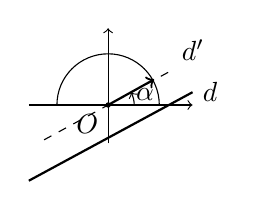
\begin{tikzpicture}[scale=0.65]
  \draw[->] (-1.55,0)--(1.65,0);
  \draw[->] (0,-0.75)--(0,1.50);
  \draw (-1,0) arc[start angle=180,end angle=0,radius=1];
  \draw[thick] (-1.55,-1.48)--(1.65,0.25) node[right] {$d$};
  \draw[dashed] (-1.25,-0.68)--(1.25,0.68) node[above right] {$d'$};
  \draw[->,thick] (0,0)--(0.9,0.5);
  \draw[->] (0.51,0) arc[start angle=0,end angle=29,radius=0.51];
  \node at (0.72,0.20) {$\alpha$};
  \fill (0,0) circle (1.5pt) node[below left] {$O$};
\end{tikzpicture}
\end{center}

\[
\begin{tikzcd}[column sep=large,row sep=large]
 \mathcal D\arrow[r,"p"]\arrow[d,"f"']
   & \mathcal D/{\sim}\arrow[dl,dashed,"\overline f"]\\
 B^1 &
\end{tikzcd}
\]
The map $f(d)$ is given as the intersection with $B^1$ of the line
through $O$ parallel to $d$.
The notes state
\[
 R_f=\sim,\qquad f\text{ is surjective},
\]
so there is a unique induced bijection
\[
 \exists!\,\overline f:\mathcal D/{\sim}\longrightarrow B^1,
 \qquad \overline f\text{ is bijective}.
\]

\medskip
\noindent\textbf{Exercise 1.}
Let $B\subseteq A$ be sets and define a relation on $\mathcal P(A)$ by
\[
 X\sim Y\iff X\cap B=Y\cap B.
\]
Show that $\sim$ is an equivalence relation and that
\[
 \mathcal P(A)/{\sim}\ \cong\ \mathcal P(B),
 \qquad X\longmapsto X\cap B.
\]

\noindent\textbf{Exercise 2.}
If $|M|=n$, calculate the number of equivalence relations
that can be defined on $M$.

\medskip
\noindent For sets $A,B$, define
\[
 A\sim B\ \overset{\mathrm{def}}{\iff}\
 \exists\,f:A\longrightarrow B\text{ bijective}.
\]
This is an equivalence relation (equipotence). The notes denote
cardinality by
\[
 \boxed{\widehat A\ \overset{\mathrm{not}}{=}
 \operatorname{card}(A)\ \overset{\mathrm{not}}{=}\ |A|}.
\]

\endgroup
